\newif\ifvimbug
\vimbugfalse

\ifvimbug
\begin{document}
\fi


\subsection{Kubische B-Splines und de Boor Algorithmus (6 Punkte)}
\subsubsection{3 Punkte}

\subsubsection{3 Punkte}

1) $1.5 \in [x_{j}, x_{j+1}) \implies 1.5 \in [1,2) \implies j=1$
\\
2) $i = j - q,...,j \implies i = -2,...,1$
\\
3) $\lambda_{1,i}^{[l]}(\xi) = \frac{x_{i+q+1-l}- \xi}{x_{i+q+1-l}-x_i}$
und $\lambda_{2,i}^{[l]}(\xi) = 1 - \lambda_{1,i}^{[l]}(\xi)$
\\
4)
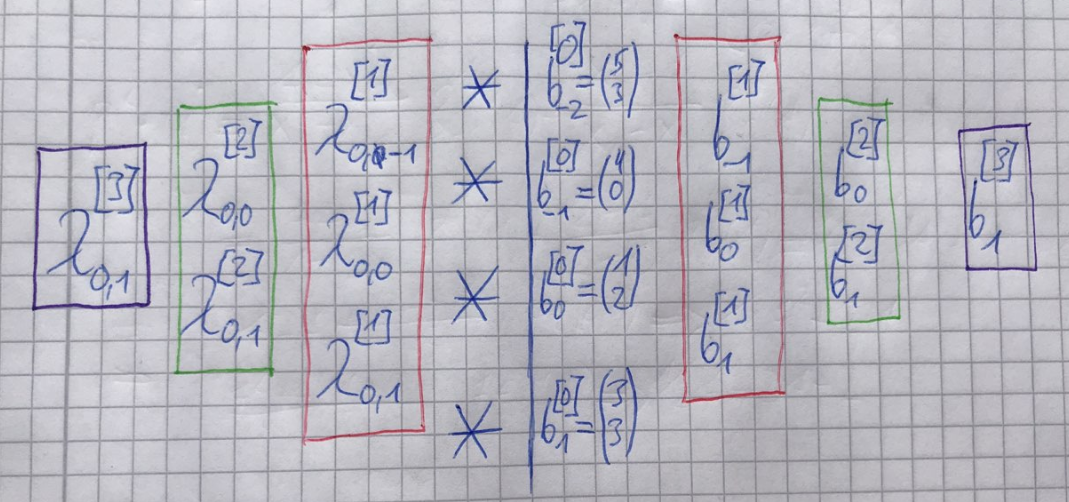
\includegraphics[scale=0.5]{1b)1.PNG}
\\
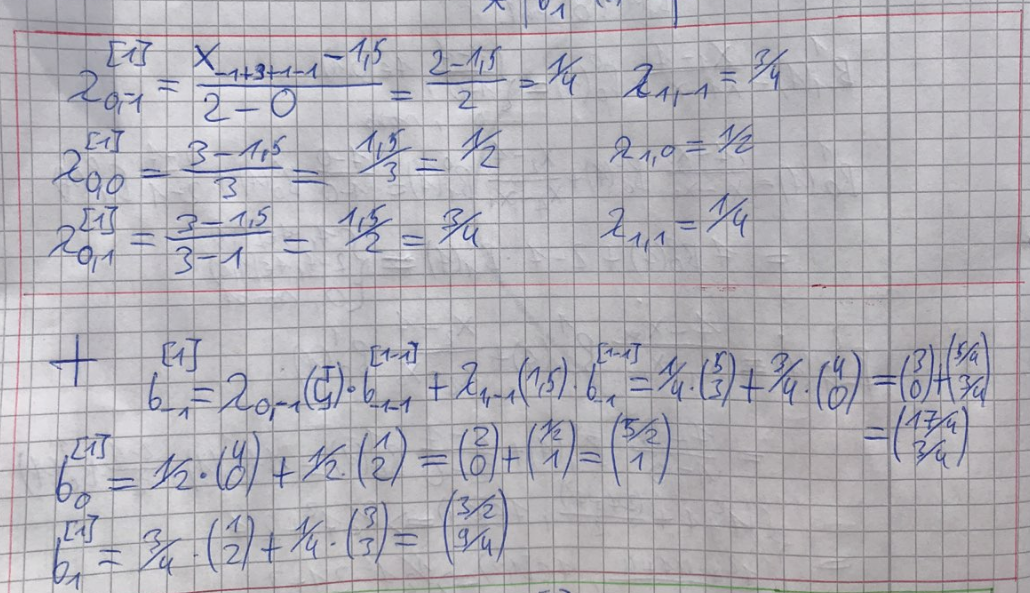
\includegraphics[scale=0.5]{1b)2.PNG}
\\
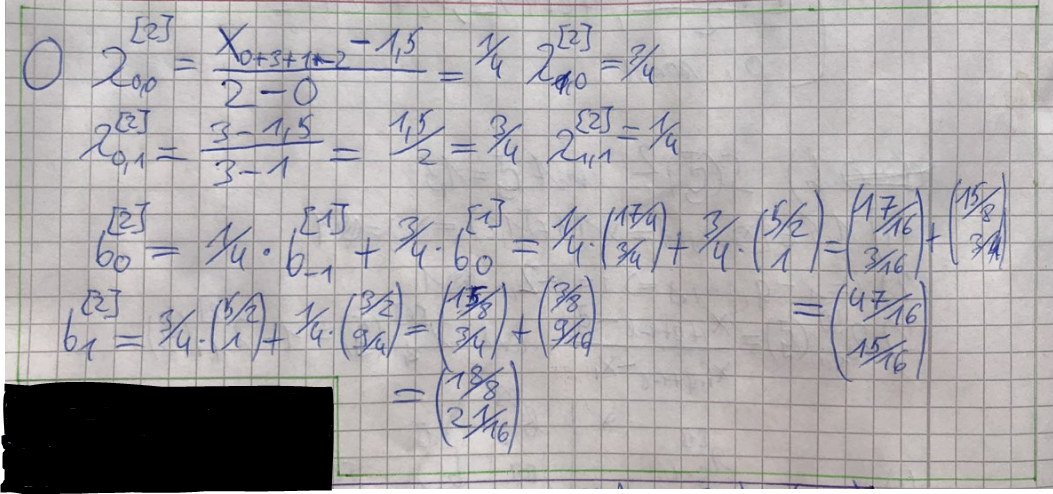
\includegraphics[scale=0.5]{1b)3.PNG}
\\
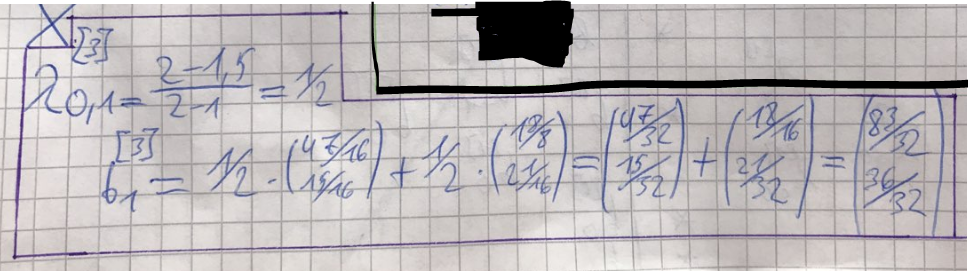
\includegraphics[scale=0.5]{1b)4.PNG}
\\
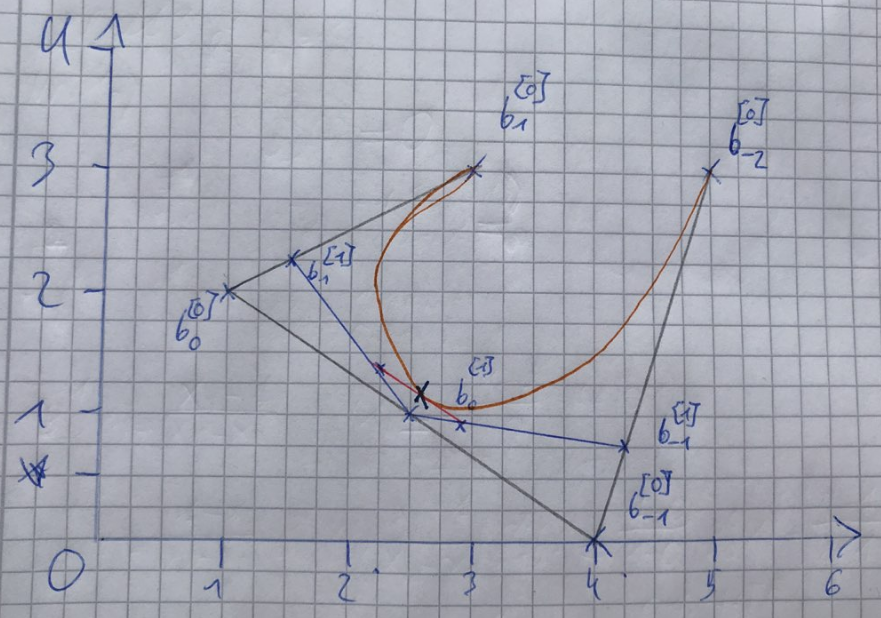
\includegraphics[scale=0.5]{1b)5.PNG}